\ifdefined\SoftwareXPublishedPreview
  \documentclass[final,5p,times,twocolumn]{elsarticle}
  \usepackage{ecrc}
  \volume{manuscript}
  \firstpage{1}
  \journalname{SoftwareX}
  \runauth{Wydaeghe et al.}
  \jid{softx}
  \jnltitlelogo{SoftwareX}
\else
  \documentclass[preprint,12pt,a4paper]{elsarticle}
\fi

\usepackage[T1]{fontenc}
\usepackage{amssymb}
\usepackage{booktabs}
\usepackage{graphicx}
\usepackage{listings}
\usepackage{tabularx}
\usepackage{xcolor}
\usepackage{hyperref}
\usepackage[acronym,nomain,nonumberlist]{glossaries}
\usepackage{microtype}
\usepackage{placeins}
\newacronym[
  longplural={Radiofrequency Electromagnetic Fields},
  shortplural={RF-EMFs}
]{rfemf}{RF-EMF}{Radiofrequency Electromagnetic Field}
\newacronym{sar}{SAR}{Specific Absorption Rate}
\newacronym{apd}{APD}{Absorbed Power Density}
\newacronym{fdtd}{FDTD}{Finite-Difference Time-Domain}
\newacronym{api}{API}{Application Programming Interface}
\newacronym{json}{JSON}{JavaScript Object Notation}
\newacronym{pifa}{PIFA}{Planar Inverted-F Antenna}
\newacronym{ifa}{IFA}{Inverted-F Antenna}
\newacronym{hdf}{HDF5}{Hierarchical Data Format Version 5}
\newacronym{cpu}{CPU}{Central Processing Unit}
\newacronym{gpu}{GPU}{Graphics Processing Unit}
\newacronym{gui}{GUI}{Graphical User Interface}
\newacronym{csv}{CSV}{Comma-Separated Values}
\newacronym{html}{HTML}{Hypertext Markup Language}
\newacronym{doi}{DOI}{Digital Object Identifier}
\newacronym{ai}{AI}{Artificial Intelligence}

\glsdisablehyper
\setlength{\parindent}{0pt}
\hypersetup{hidelinks}

\journal{SoftwareX}
\frenchspacing

\lstdefinestyle{goliat}{
  basicstyle=\ttfamily\small,
  frame=single,
  framerule=0.5pt,
  rulecolor=\color{black},
  columns=fullflexible,
  keepspaces=true,
  showstringspaces=false,
  breaklines=true,
  aboveskip=6pt,
  belowskip=6pt
}

\begin{document}
\renewcommand{\labelenumii}{\arabic{enumi}.\arabic{enumii}}

\begin{frontmatter}

\ifdefined\SoftwareXPublishedPreview
\dochead{Original Software Publication}
\fi

\title{GOLIAT: A configurable workflow for near- and far-field\\ RF-EMF dosimetry in Sim4Life}

\author[ugent]{Robin Wydaeghe\corref{cor1}}
\ead{robin.wydaeghe@ugent.be}
\author[ugent]{Emmeric Tanghe}
\author[ugent]{Wout Joseph}
\cortext[cor1]{Corresponding author}

\address[ugent]{Department of Information Technology, Ghent University--imec, WAVES Research Group, Technologiepark-Zwijnaarde 126, 9052 Ghent, Belgium}

\begin{abstract}
GOLIAT is an open-source Python framework for Radiofrequency Electromagnetic Field (RF-EMF) dosimetry with Sim4Life. Users define phantoms, sources, exposure cases, numerical settings, and requested outputs in hierarchical JavaScript Object Notation (JSON) files. GOLIAT supports both near-field and far-field simulation studies. The software sets up each scene, runs each job locally, across workers, or through oSPARC, extracts Specific Absorption Rate (SAR) and Absorbed Power Density (APD), and writes campaign tables and plots. GOLIAT has supported 352 near-field simulations across two child phantoms, eight frequencies, and 22 placements at each phantom--frequency pair, and 550 far-field simulations across four phantoms and 15 frequencies.
\end{abstract}

\begin{keyword}
RF-EMF dosimetry \sep specific absorption rate \sep absorbed power density \sep finite-difference time-domain \sep simulation workflow \sep Sim4Life
\end{keyword}

\end{frontmatter}

\ifdefined\SoftwareXPublishedPreview
\else
\clearpage
\section*{Metadata}
\fi

\begin{table*}[!ht]
\centering
\small
\begin{tabularx}{\textwidth}{|l|>{\raggedright\arraybackslash}p{0.34\textwidth}|>{\raggedright\arraybackslash}X|}
\hline
\textbf{Nr.} & \textbf{Code metadata description} & \textbf{Metadata} \\
\hline
C1 & Current code version & v1.5.0 \\
\hline
C2 & Permanent link to code/repository used for this code version & \url{https://github.com/rwydaegh/goliat/releases/tag/v1.5.0} \\
\hline
C3 & Permanent link to Reproducible Capsule & Not available. Full solver execution requires a commercial Sim4Life license. \\
\hline
C4 & Legal Code License & Apache License 2.0 \\
\hline
C5 & Code versioning system used & git \\
\hline
C6 & Software code languages, tools, and services used & Python 3.11, Sim4Life Python \gls{api}, PySide6, and oSPARC \gls{api} \\
\hline
C7 & Compilation requirements, operating environments \& dependencies & Python 3.11; Microsoft Windows for local Sim4Life execution; Sim4Life 8.2 or 9.2; Python dependencies declared in \texttt{pyproject.toml}; optional oSPARC access \\
\hline
C8 & If available Link to developer documentation/manual & \url{https://docs.goliat.waves-ugent.be/} \\
\hline
C9 & Support email for questions & \url{robin.wydaeghe@ugent.be} \\
\hline
\end{tabularx}
\caption{Code metadata (mandatory).}
\label{codeMetadata}
\end{table*}

\glsresetall

\section{Motivation and significance}

Computational \gls{rfemf} dosimetry calculates energy absorption in the body with numerical models. The main quantities are whole-body and local \gls{sar} below 6~GHz and \gls{apd} at higher frequencies~\cite{Hand2008,Hirata2021}. A study may vary the anatomical model, frequency, source position, incident direction, polarization, grid, and normalization. Together, these choices can give hundreds of \gls{fdtd} simulations.

Each simulation needs a scene, source, material assignment, grid, boundary conditions, solver settings, sensors, and extraction rules. A campaign also needs consistent names, result paths, normalization, and summary tables. Manual projects work well for a small study. However, large parameter sets need the same case setup and result collection each time.

Sim4Life has anatomical models, electromagnetic solvers, dosimetry evaluators, a graphical interface, and a Python \gls{api}~\cite{Gosselin2014,Sim4Life}. The \gls{api} can automate one simulation. However, a study script must still list cases, name project and result files, select phases for reruns, and combine results. If one script has both the rules and scientific parameters, reviewers must read and edit program code to check or reuse the study.

GOLIAT has one workflow for study definition, scene setup, execution, extraction, and analysis. Users set scientific and numerical choices in hierarchical \gls{json} files. A base file has shared settings. Users set the phantoms, sources, exposure cases, grids, and outputs in smaller study files. GOLIAT validates the merged configuration and writes one expanded configuration for each simulation job. Users can review these files before a run and store them with the results~\cite{Sandve2013,Wilson2014}.

Near- and far-field studies use different scene rules. A near-field case places an antenna relative to an anatomical landmark and uses an input-power normalization. A far-field case defines incident fields, directions, and polarizations and uses an incident-power-density normalization. Both study types use the same job identity, execution interface, output layout, and campaign analysis.

GOLIAT uses the Sim4Life solver and evaluators. Table~\ref{tab:capabilities} lists its study-level functions.

\begin{table*}[!ht]
\centering
\small
\begin{tabularx}{\textwidth}{@{}>{\raggedright\arraybackslash}p{0.17\textwidth}>{\raggedright\arraybackslash}p{0.48\textwidth}>{\raggedright\arraybackslash}X@{}}
\toprule
Study task & GOLIAT function & Main output \\
\midrule
Define a study & Inherited and validated \gls{json} for phantoms, sources, numerical controls, and requested metrics & Expanded configuration per job \\
Set up near-field scenes & Antenna import, material mapping, and eye, cheek, trunk, or wrist placement relative to anatomical landmarks & Isolated device--body project \\
Set up far-field scenes & Plane-wave or beamforming sources over direction and polarization sets & Isolated incident-field project \\
Run simulations & Local \texttt{iSolve}, split workers, multiple workstations, or oSPARC batch jobs & Solver output, logs, and progress record \\
Extract dosimetry & Whole-body, regional, tissue, and peak 10~g \gls{sar}, \gls{apd}, point fields, and power balance & \gls{json}, serialized tissue table, and \gls{html} report \\
Analyze a campaign & Shared result discovery, normalization, grouping, and plotting & Detailed and summary \gls{csv}, Excel, and plots \\
Manage jobs & Per-job projects, status records, deliverable checks, and optional phase recovery & Reviewable scenario directory \\
\bottomrule
\end{tabularx}
\caption{Main GOLIAT functions and outputs.}
\label{tab:capabilities}
\end{table*}

\section{Software description}

\subsection{Software architecture}

Figure~\ref{fig:flowchart} shows the main components. The command-line interface loads and validates a configuration and selects a near-field or far-field study class. Both study classes use the same project manager, execution interface, status reporting, profiling, and directory layout. Exposure-specific setup and analysis classes define the geometry, source, normalization, and grouping rules.

\begin{figure*}[!ht]
  \centering
  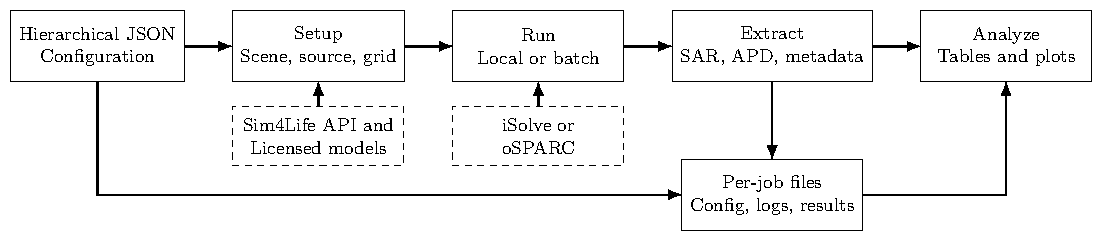
\includegraphics[width=\textwidth]{workflow.pdf}
  \caption{GOLIAT flowchart from a hierarchical study definition to campaign tables and plots. The near- and far-field study classes share project, execution, extraction, and analysis interfaces. Dashed boxes mark external Sim4Life, model, and oSPARC resources.}
  \label{fig:flowchart}
\end{figure*}

A base configuration has common solver settings, output quantities, material rules, and paths. A derived file sets the values for one study. The loader merges the files and validates the result before scene construction. Study classes then make one job for each parameter combination.

First, setup classes set the geometry, materials, sources, grids, boundary conditions, and sensors for each job. Second, GOLIAT runs jobs with \texttt{iSolve}, the Sim4Life \gls{api}, or oSPARC. Third, extractors write common result files from Sim4Life and \gls{hdf} outputs. Finally, analysis strategies read those files without reopening every Sim4Life project.

The package keeps exposure rules separate from project and result management. Therefore, a new study type can use the common interfaces with its own setup and extraction rules.

\subsection{Software functionalities}

\subsubsection{Study definition and scene setup}

Near-field configurations select \gls{pifa} or \gls{ifa} models by frequency. Each antenna part has a material and grid setting. The anatomical landmarks are the nasion, tragus, and umbilicus. The nasion is the midline depression at the bridge of the nose. The tragus is the cartilage projection in front of the ear canal. The umbilicus is the navel. Users can define eye, cheek, trunk, wrist, or free-space cases with offsets and rotation sequences. The setup code loads the phantom and antenna, places the antenna, sets the simulation domain and grid, and writes the solver input.

Users set the far-field source type, incident directions, polarizations, and frequencies. For example, spherical tessellation gives a configurable set of incident directions. A multi-sine source runs configured frequencies together. The extractor keeps each frequency component. Grid controls can set frequency-specific steps, domain padding, high-frequency phantom truncation, and bilateral symmetry. The auto-induced workflow combines environmental field results, ranks candidate focus points, and extracts the selected high-exposure cases.

Both study types have settings for solver termination, excitation, boundaries, padding, sensors, kernels, and grids. Users can choose automatic grids or set manual steps for the whole domain and selected components. The configuration also selects the requested result quantities and tissue groups.

\subsubsection{Execution and monitoring}

Local execution calls the Sim4Life \texttt{iSolve} executable and records its output. Split execution divides one configuration into disjoint job sets for \gls{cpu} processes or separate workstations. Setup and extraction can use several \gls{cpu} processes. However, \gls{fdtd} solves remain serial on a single-\gls{gpu} workstation. oSPARC execution writes solver inputs, submits batch jobs, monitors their states, retries failed submissions, and downloads the outputs~\cite{oSPARC}.

A PySide6 interface shows the active phase, completed jobs, time estimates, logs, and \gls{cpu}, memory, and \gls{gpu} use. A console mode provides the same study commands without the interface. GOLIAT uses timing records for phase estimates and campaign statistics. Progress and verbose logs remain available after the session.

Each job has a separate Sim4Life project and result directory. GOLIAT records phase status, checks project locks and required deliverables, and retries failed saves or remote submissions. Users can rerun setup, solving, or extraction for selected jobs. A checksum identifies changes to the expanded configuration. The job record can also store the GOLIAT release, Sim4Life version, model identifiers, and material data.

\subsubsection{Extraction and analysis}

GOLIAT extracts whole-body, head, trunk, tissue-specific, and peak spatial-average \gls{sar} over 10~g. It also extracts point-sensor fields and power balance. High-frequency studies can request \gls{apd} over a selected averaging area. Near-field results use the declared antenna input power. Far-field results use the incident power density.

Each scenario directory can have the project, solver input and output, expanded configuration, logs, a compact \texttt{sar\_results.json}, a serialized tissue table, an \gls{html} report, and simulation metadata. The metadata record timings, solver settings, grid size, hardware, performance, power balance, and file sizes.

The analysis command finds completed scenario directories and writes detailed and summary \gls{csv} files, Excel workbooks, and plots. GOLIAT can make heatmaps, line charts, bar charts, boxplots, cumulative distributions, power summaries, and tissue rankings. Near- and far-field analysis classes use the same file discovery and export rules. A paper-generation command can place selected tables and plots in a LaTeX results draft.

The package has commands for studies, validation, analysis, status, initialization, and parallel execution. A typical command sequence is:

\noindent\begin{minipage}{\linewidth}
\begin{lstlisting}[style=goliat]
goliat validate far_field_config
goliat study far_field_config
goliat analyze far_field_config
\end{lstlisting}
\end{minipage}

The documentation has installation instructions, five tutorial notebooks, configuration references, an \gls{api} reference, cloud instructions, and troubleshooting notes~\cite{GOLIATDocs}. The Apache-2.0 package is available on PyPI~\cite{GOLIATPyPI}.

\section{Illustrative examples}

The examples come from two completed campaigns: device-to-body and far-field exposure. The far-field campaign has environmental and auto-induced cases. Figure~\ref{fig:configuration} shows the parameters that differ between the two study types. The job record and analysis interface remain the same.

\begin{figure*}[!ht]
  \centering
  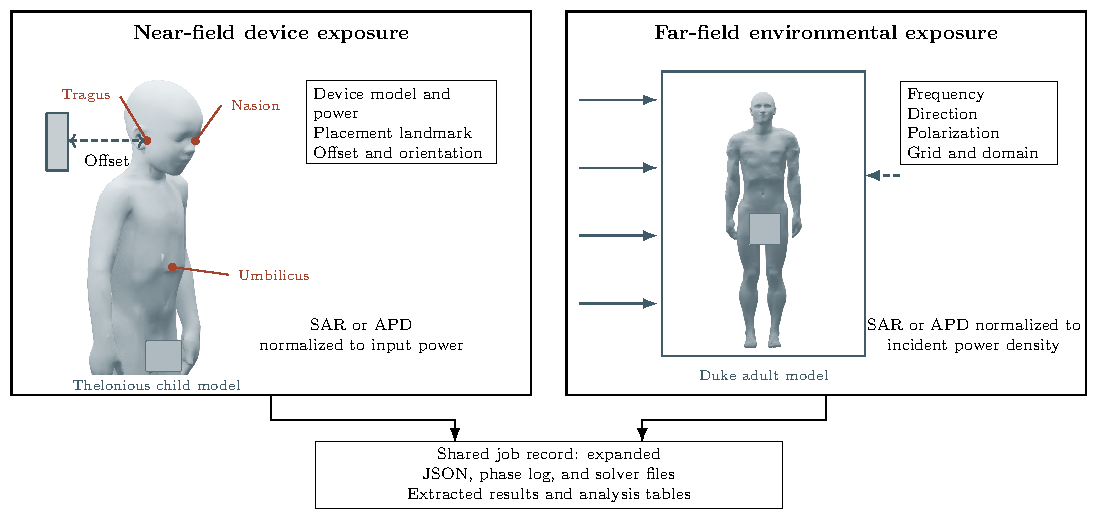
\includegraphics[width=0.92\textwidth]{exposure_modes.pdf}
  \caption{Near- and far-field paths with the Thelonious and Duke anatomical surface meshes~\cite{Gosselin2014}. Markers identify the nasion, tragus, and umbilicus used for device placement. Device cases use input-power normalization. Environmental cases use plane-wave directions, polarizations, and incident-power-density normalization. Both paths produce the same job record.}
  \label{fig:configuration}
\end{figure*}

\subsection{Near-field device campaign}

The near-field study used two child phantoms, eight frequencies from 700~MHz to 5.8~GHz, and 22 device placements per phantom and frequency. The study used \gls{pifa} models at 700 and 835~MHz and \gls{ifa} models at the other six frequencies. The study used eight eye, six cheek, and eight belly placements. Eye and belly cases varied position and horizontal or vertical orientation. Cheek cases used cheek and tilt alignments with three angular variants.

Thus, GOLIAT expanded the study into $2\times8\times22=352$ simulation jobs. All 352 scenario directories have an expanded configuration, progress and solver logs, compact \gls{sar} results, a serialized tissue table, and an \gls{html} report. Figure~\ref{fig:near-field-campaign} shows complete coverage for both phantoms and the recorded solver time by frequency. One cell-iteration is one grid cell advanced through one \gls{fdtd} time step.

\begin{figure*}[!ht]
  \centering
  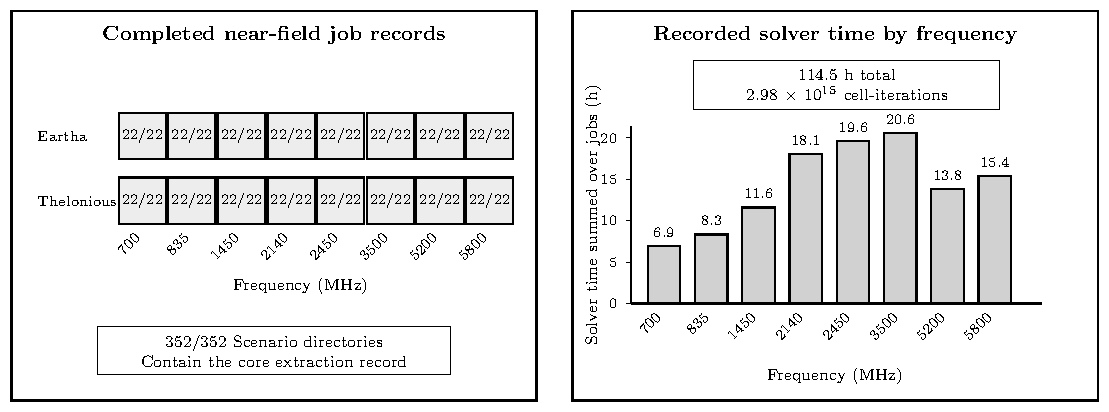
\includegraphics[width=0.95\textwidth]{near_field_campaign.pdf}
  \caption{Executed near-field campaign. Each phantom--frequency cell contains 22 completed device placements. The solver logs record 114.5 cumulative hours and $2.98\times10^{15}$ cell-iterations across the 352 jobs. The total time uses the unrounded per-job values.}
\label{fig:near-field-campaign}
\end{figure*}

The configuration set the antenna model, target input power, material mapping, grid rules, anatomical reference, distance, position, and orientation for each case. GOLIAT generated the Sim4Life scene and normalized extracted \gls{sar} values to the declared input power. The analysis step grouped results by phantom, frequency, placement, and tissue. It produced detailed tables and several plot families.

\subsection{Far-field research campaign}

GOLIAT supported a far-field campaign with two adult and two child Virtual Population phantoms~\cite{Gosselin2014,GOLIATFarField}. The study covered 15 frequencies from 450~MHz to 26~GHz and produced 550 \gls{fdtd} simulations in Sim4Life 8.2. Environmental exposure used incident plane waves. Auto-induced exposure used a beamforming source model. The scientific results and numerical methods are reported in the \emph{Physics in Medicine \& Biology} article~\cite{GOLIATFarField}.

The environmental sub-study below 6~GHz had four phantoms, nine frequencies, six incident directions, and two polarizations. Therefore, GOLIAT generated all 432 parameter combinations. Base files stored shared execution, material, extraction, and output settings. Derived files selected environmental and beamforming cases. The full campaign added higher-frequency and auto-induced cases.

GOLIAT stored each job in a separate project and result directory. The path encoded the study, phantom, frequency, and exposure case. Figure~\ref{fig:run-directory} shows one completed environmental job. The completed job directory has its configuration and extracted results beside the project and solver files. Operators can inspect, transfer, or reprocess each job separately.

\begin{figure*}[!ht]
  \centering
  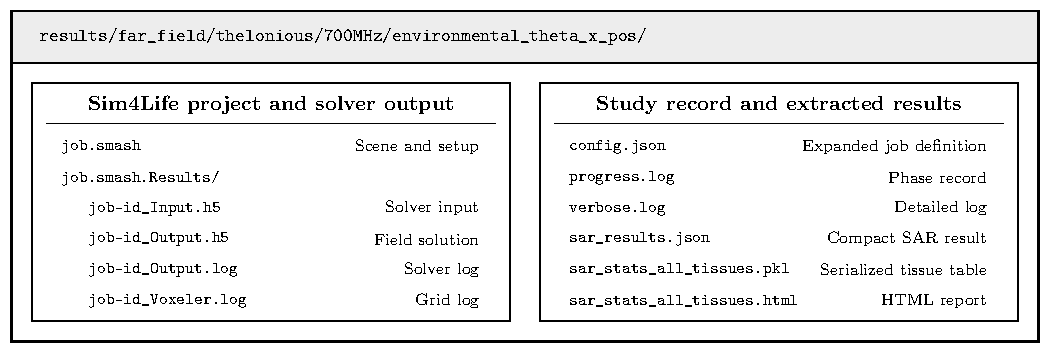
\includegraphics[width=0.95\textwidth]{run_directory.pdf}
  \caption{Representative files for one completed far-field job. File identifiers are shortened. Each scenario contains the Sim4Life project and solver output, expanded configuration, logs, and compact \gls{sar} results.}
  \label{fig:run-directory}
\end{figure*}

Figure~\ref{fig:monitoring-output} shows two outputs from the documented workflows. The monitoring page shows phase progress and the live worker log. Extraction writes the point-sensor plot to the job results.

\begin{figure*}[!ht]
  \centering
  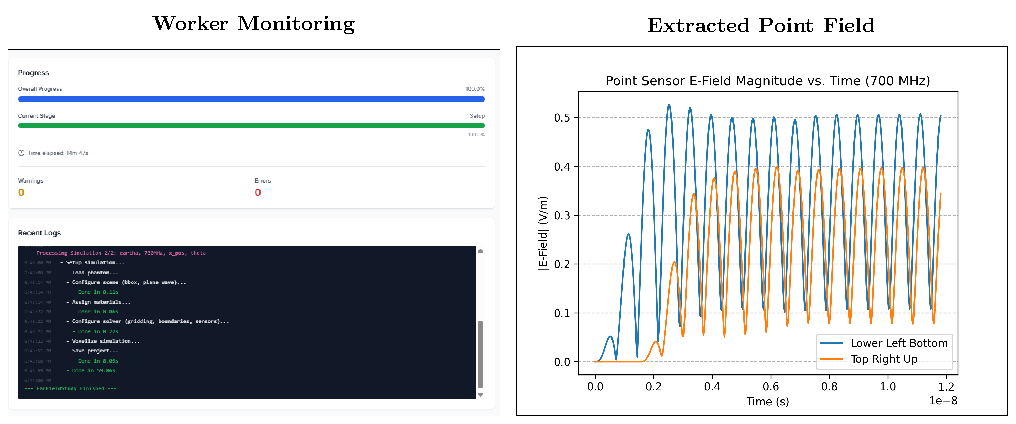
\includegraphics[width=0.94\textwidth]{monitoring_and_output.pdf}
  \caption{Documented software outputs. Left: web monitoring for one worker after scene setup. Right: extracted point-sensor electric-field traces for a 700~MHz tutorial case.}
  \label{fig:monitoring-output}
\end{figure*}

The campaign analysis read the same directory structure for all 550 jobs and wrote scenario, frequency, and tissue tables. The Harvard Dataverse deposit contains consolidated configurations and postprocessed \gls{sar} and \gls{apd} data~\cite{GOLIATFarFieldData}. Licensed anatomical models and raw solver projects are excluded.

Table~\ref{tab:evidence} lists the evidence used for the software claims. The near-field and far-field campaigns together have 902 completed \gls{fdtd} job records.

\begin{table*}[!ht]
\centering
\small
\begin{tabularx}{\textwidth}{@{}>{\raggedright\arraybackslash}p{0.22\textwidth}>{\raggedright\arraybackslash}p{0.28\textwidth}>{\raggedright\arraybackslash}X@{}}
\toprule
Evidence source & Scope & Observed record \\
\midrule
Repository continuous integration & Configuration checks and license-free automated tests & GitHub Actions completed these tests on source commit \texttt{23f0ce8}. \\
Near-field licensed execution & Two phantoms, eight frequencies, and 22 placements & All 352 expected directories contain the expanded configuration, logs, and core \gls{sar} extraction files. \\
Far-field environmental expansion & Four phantoms, nine frequencies, six directions, and two polarizations & The configuration produced 432 per-scenario directories below 6~GHz. \\
Far-field licensed execution & Environmental and auto-induced sub-studies over 15 frequencies & The analysis command read 550 scenario records and generated the campaign tables supplied to the \emph{Physics in Medicine \& Biology} article~\cite{GOLIATFarField}. \\
\bottomrule
\end{tabularx}
\caption{Configuration, execution, and output evidence used in this paper.}
\label{tab:evidence}
\end{table*}

Common settings appear once in the base configuration. Source, frequency, and study choices remain in smaller derived files. Reviewers can compare those files and locate changes to a grid, source, phantom subset, or extraction metric. The result tables keep the case coordinates used for the comparison.

\FloatBarrier
\section{Impact}

GOLIAT was developed for the European GOLIAT project and has supported two large computational dosimetry campaigns. The near-field campaign produced 352 device-exposure simulations for two child phantoms. The far-field campaign produced 550 environmental and auto-induced simulations for four child and adult phantoms~\cite{GOLIATFarField}. Both campaigns used the same configuration, job directory, extraction, and analysis structure.

Researchers can add a phantom, frequency, incident direction, polarization, or device placement without changing the common execution and output interfaces. Configuration inheritance keeps shared settings in one base file. Derived files show the choices that differ between studies. The same analysis code can then group results by phantom, source, frequency, exposure case, and tissue.

GOLIAT runs job sets on one workstation, across separate workers, or through oSPARC. A workstation can call \texttt{iSolve}. oSPARC can run independent solver jobs in parallel. The \gls{gui} and logs give the operator a common view of each route.

Test laboratories and device developers can use a controlled GOLIAT configuration as a computational profile. IEC/IEEE~62704-3 defines \gls{fdtd} procedures, benchmark phone models, meshing guidance, test positions, uncertainty, and validation for mobile-phone \gls{sar} pre-compliance from 30~MHz to 6~GHz~\cite{IEC627043}. IEC/IEEE~63195-2:2022 defines computational incident-power-density procedures for devices used within 200~mm of the head or body from 6 to 300~GHz~\cite{IEC631952}. IEEE/IEC P63195-4 is an active project for computational absorbed-power-density procedures in the same frequency range~\cite{IEEEP631954}.

IEC/IEEE~62704-3 provides the procedural basis for near-field \gls{sar} profiles below 6~GHz. A profile can fix device-to-head or device-to-trunk placements, input power, frequencies, grid rules, and \gls{sar} fields. Above 6~GHz, IEC/IEEE~63195-2 covers incident power density, while the active IEEE/IEC P63195-4 project covers absorbed power density. GOLIAT can store the grid and output settings used with these procedures.

Far-field environmental profiles are for research and internal repeatability unless a separate assessment procedure defines them. A far-field profile can set anatomical models, incident directions, polarizations, normalization, and report fields.

A test laboratory can place a GOLIAT configuration and its job records under change control for repeated pre-compliance studies. The profile gives each device revision the same scenario coordinates and report fields. The configuration diff records changes to the computational procedure. A complete record also lists release identifiers, model identifiers, the material database, and the solver version.

The laboratory must also qualify device and phantom models, validate the numerical setup, analyze uncertainty, control releases, and follow its quality system. GOLIAT records the selected grid, material set, exposure case, and normalization. Users can use power balance, logs, and metadata to flag suspect runs and review the model setup.

However, local scene setup and solver execution require a licensed Sim4Life installation on Windows. The source release does not contain licensed anatomical models. Users must obtain them under the applicable license. Continuous integration can test configuration handling, job management, and analysis code without Sim4Life. Full \gls{fdtd} reproduction still needs the solver and the selected models. Sim4Life version changes need \gls{api} and numerical regression checks.

\section{Conclusions}

GOLIAT uses hierarchical \gls{json} study definitions to create near- and far-field Sim4Life jobs and common analysis-ready results. The completed campaigns have 352 near-field and 550 far-field jobs with configurations, logs, and extracted results. Laboratories can use a controlled profile for repeatable research and pre-compliance studies after they qualify the models, validate the numerical setup, analyze uncertainty, control releases, and follow their quality procedures.

\section*{Funding}

The GOLIAT project has received funding from the European Union's Horizon Europe research and innovation programme under grant agreement No.~101057262. Views and opinions expressed are those of the authors only and do not necessarily reflect those of the European Union or the European Health and Digital Executive Agency. Neither the European Union nor the granting authority can be held responsible for them.

\section*{CRediT authorship contribution statement}

Robin Wydaeghe: Conceptualization, Methodology, Software, Validation, Formal analysis, Investigation, Data curation, Writing -- original draft, Visualization. Emmeric Tanghe: Conceptualization, Methodology, Supervision, Writing -- review \& editing. Wout Joseph: Conceptualization, Supervision, Funding acquisition, Project administration, Writing -- review \& editing.

\section*{Declaration of competing interest}

The authors declare no competing financial interests or personal relationships that could have influenced the work reported in this paper.

\section*{Declaration of generative \glsentryshort{ai} and \glsentryshort{ai}-assisted technologies in the writing process}

During preparation of this work, the authors used \gls{ai} for language editing and preparation of the paper figures. The authors reviewed and edited the text and checked the software claims. The authors take full responsibility for the article.

\section*{Data availability}

The code release is identified in Table~\ref{codeMetadata}. The postprocessed data and configuration family for the far-field example are deposited in Harvard Dataverse under \gls{doi} 10.7910/DVN/EEEE0X~\cite{GOLIATFarFieldData}. The paper-release archive has a 352-row near-field job manifest and the solver summary used in Figure~\ref{fig:near-field-campaign}. Neither archive has licensed Virtual Population phantoms or Sim4Life project files.

\section*{Acknowledgements}

The authors thank Bryn Lloyd of ZMT Zurich MedTech AG for feedback through GitHub issues and pull requests. They also thank him for supporting GOLIAT's addition to the official oSPARC client documentation and for proposing its addition to the official Sim4Life documentation.

\bibliographystyle{elsarticle-num}
\bibliography{references}

\end{document}
